
\documentclass{thesisclass}
\usepackage[toc,page]{appendix}
\usepackage{pdfpages} 
\usepackage{pgfplots}
\pgfplotsset{compat=1.8}
\usepgfplotslibrary{statistics}
\usepackage{filecontents}
\pgfplotsset{width=7cm,compat=1.16}
\pgfplotsset{
boxplot/every box/.style={solid, black},
boxplot/every whisker/.style={solid, black},
boxplot/every median/.style={solid, black},
every boxplot/.style={mark=diamond*, every mark/.append style={black}}
}

\makeindex
% Based on thesisclass.cls of Timo Rohrberg, 2009
% ----------------------------------------------------------------
% Thesis - Main document
% ----------------------------------------------------------------


%% -------------------------------
%% |  Information for PDF file   |
%% -------------------------------
\hypersetup{
 pdfauthor={},
 pdftitle={},
 pdfsubject={Not set},
 pdfkeywords={Not set}
}

\newcommand{\tm}{\textsuperscript{\scriptsize\texttrademark}}
\newcommand{\reg}{\textsuperscript{\scriptsize\textregistered}}
\renewcommand{\appendixtocname}{Anhang}
\renewcommand{\appendixpagename}{Anhang}
%\newcommand{\copy}{\textsuperscript{\scriptsize\textcopyright}}

%% ---------------------------------
%% | Information about the thesis  |
%% ---------------------------------

\newcommand{\myname}{Antonia Gerdes}
\newcommand{\mytitle}{Holographische Visualisierung der Leber mit markergestütztem Tracking an einem Phantom}

\newcommand{\reviewerone}{Prof. Dr.-Ing. Stefanie Speidel}
\newcommand{\reviewertwo}{Dr.-Ing. Sebastian Bodenstedt}
\newcommand{\advisor}{Micha Pfeiffer}
% If there is a second advisor, uncomment in titlepage.tex!
\newcommand{\advisortwo}{?}

\newcommand{\timestart}{Juli 08, 2019}
\newcommand{\timeend}{September 23, 2019}
\newcommand{\submissiontime}{19. Monat 20XX}


%% ---------------------------------
%% | ToDo Marker - only for draft! |
%% ---------------------------------
% Remove this section for final version!
%\setlength{\marginparwidth}{20mm}


%% --------------------------------
%% | Settings for word separation |
%% --------------------------------
% Help for separation:
% In german package the following hints are additionally available:
% "- = Additional separation
% "| = Suppress ligation and possible separation (e.g. Schaf"|fell)
% "~ = Hyphenation without separation (e.g. bergauf und "~ab)
% "= = Hyphenation with separation before and after
% "" = Separation without a hyphenation (e.g. und/""oder)

% Describe separation hints here:
\hyphenation{
% Pro-to-koll-in-stan-zen
% Ma-na-ge-ment  Netz-werk-ele-men-ten
% Netz-werk Netz-werk-re-ser-vie-rung
% Netz-werk-adap-ter Fein-ju-stier-ung
% Da-ten-strom-spe-zi-fi-ka-tion Pa-ket-rumpf
% Kon-troll-in-stanz
}

%%%%%%%%%%%%%%%%%%%%%%%%%%%%%%%%%
%% Here, main documents begins %%
%%%%%%%%%%%%%%%%%%%%%%%%%%%%%%%%%
\begin{document}

% Uncomment the following line for English text
%\selectlanguage{english}
\frontmatter
\pagenumbering{roman}

% Coordinates for the bg shape on the titlepage
\newcommand{\xone}{-15}
\newcommand{\xtwo}{\textwidth+15}
\newcommand{\yone}{15}
\newcommand{\ytwo}{-212}
\newcommand{\ythree}{-253}
\newcommand{\rounded}{2}	% radius of rounded corners

% Colors:
\definecolor{nct_blue}{rgb}{0,0.09,0.43}
\definecolor{nct_light_blue}{rgb}{0.2,0.45,0.76}

\begin{titlepage}
	
	\begin{tikzpicture}[overlay]
	\draw[color=nct_blue, semithick, rounded corners=\rounded mm]
		(\xone mm, \yone mm) rectangle (\xtwo mm, \ythree mm);
	\end{tikzpicture}
	

	\changefont{phv}{m}{n}	% helvetica
	\vspace*{2.5cm}
	\begin{center}
		\Huge{\mytitle}
		\vspace*{1.5cm}
		\\
		\Large{
			\iflanguage{english}{Master Thesis}												  {Masterarbeit}
		}\\
		\vspace*{1cm}
		\huge{\myname}
		\\
		\vspace*{1cm}
		\Large{
			\iflanguage{english}{Division Translational Surgical Oncology\\NCT Dresden}
								{Abteilung Translationale Chirurgische Onkologie\\NCT Dresden}
		}
		
	\end{center}
	\vspace*{1cm}
	\Large{
	\begin{center}
	\begin{tabular}[ht]{l c l}
	  % Gutachter sind die Professoren, die die Arbeit bewerten.
	  \iflanguage{english}{Reviewer}{Erstgutachter}: & \hfill  & \reviewerone\\
	  \iflanguage{english}{Second reviewer}{Zweitgutachter}: & \hfill  & \reviewertwo\\
	  \iflanguage{english}{Advisor}{Betreuender Mitarbeiter}: & \hfill  & \advisor\\
	  % Uncomment the following line if there is a second advisor:
	  %\iflanguage{english}{Second advisor}{Zweiter betreuender Mitarbeiter}: & \hfill  & \advisortwo\\
	\end{tabular}
	\end{center}
	}
	
	\begin{center}
	\vspace{\baselineskip}
	\large{\iflanguage{english}{Duration}{Bearbeitungszeit}: \timestart \hspace*{0.25cm} -- \hspace*{0.25cm} \timeend}
	\end{center}	
	
	\begin{textblock}{10}[0,0](4.1,14.8)
		\iflanguage{english}{
				\includegraphics[width=.65\textwidth]{images/logos/NCT_Dresden_zweispaltig_englisch.pdf}
			}{
				\includegraphics[width=.67\textwidth]{images/logos/NCT_Dresden_zweispaltig.pdf}
			}
	\end{textblock}
	\begin{textblock}{10}[0,0](11.7,14.8)
		%\raggedleft		% Shift to the left
		\includegraphics[width=.4\textwidth]{images/logos/TU_Dresden_Logo_HKS41.pdf}
	\end{textblock}

\end{titlepage}

\blankpage
\renewcommand{\figurename}{Abb.}

\thispagestyle{empty}
$\mbox{}$\vspace{15cm}$\mbox{}$\\
Ich versichere hiermit, die vorliegende Arbeit selbstständig angefertigt zu haben. Die verwendeten Hilfsmittel und Quellen sind im Literaturverzeichnis
vollständig aufgeführt.\\
$\mbox{}$\vspace{2cm}$\mbox{}$\\
Dresden, den 03. September, 2019\\
$\mbox{}$\vspace{1cm}$\mbox{}$\\
$\mbox{}$\hfill \\
$\mbox{}$


\clearpage

% blank page
\newpage
\hfill
\thispagestyle{empty}

% abstract
\newpage
\thispagestyle{empty}
\chapter*{\centering \iflanguage{english}{Abstract}{Zusammenfassung}}

\emph{Augmented Reality} (AR) bietet große Chancen im medizinischen Bereich. Sowohl in der minimalinvasiven, als auch der offenen Chirurgie ist es möglich, Chirurgen durch Augmented Reality zu unterstützen. Auch im Training angehender Chirurgen können AR-Systeme eingesetzt werden. \emph{Head Mounted Displays} (HMDs) ermöglichen das Anzeigen von Daten im Sichtfeld des Chirurgen, ohne dass dieser den Blick vom Patienten abwenden muss.

\textbf{Methoden:} Ziel dieser Arbeit ist das Visualisieren der Leber an einem Phantom mit Hilfe von Augmented Reality ohne ein externes Trackingsystem. Die Visualisierung erfolgt mit Hilfe eines Head Mounted Displays und Tracking von \emph{Fiducials} an einem Phantom. Mit Hilfe der Fiducials wird die Lage des Phantoms im Raum bestimmt. Dazu muss der Offset zwischen Fiducials und Phantom bekannt sein. Zusätzlich wird ein Vorgehen zur Kalibrierung des Offsets der Fiducials entwickelt.

\textbf{Evaluation:} Es wurde zur Evaluation eine Nutzerstudie durchgeführt. Die Probanden sollten eigenständig den Offset zwischen Fiducials und Phantom kalibrieren. Anschließend bewerteten sie ihre Kalibrierung und verglichen sie mit einer über ein externes Trackingsystem durchgeführte Kalibrierung. Die Kalibrierungen der Probanden wurden quantitativ ausgewertet.

\textbf{Diskussion:} Das Ziel der Arbeit, ein 3D-Modell des Phantoms mit dem realen Objekt zu registrieren, wurde erreicht. Es konnte zum Tracken von Phantom und Hololens auf ein externes Trackingsystem verzichtet werden. Auch bei der Kalibrierung war es möglich, auf ein externes Trackingsystem zu verzichten.
Durch Limitierungen in der Hardware, der Probanden und durch die nur prototypische Umsetzung der Anwendung war dennoch die Kalibrierung mit Hilfe eines externen Trackingsystems genauer. Es ist jedoch vorstellbar, dass mit den genannten Ansätzen zur Verbesserung der Anwendung ein ebenso gutes Ergebnis in der Kalibrierung mit der Hololens in Zukunft möglich ist.


\newpage

\newpage
\hfill
\thispagestyle{empty}

% toc
\newpage
\thispagestyle{empty}
\tableofcontents
\newpage
\setcounter{page}{1}

% blank page
\newpage
\hfill
\thispagestyle{empty}
\hfill
\newpage

%% -----------------
%% |   Main part   |
%% -----------------
%add content here
%it is preferable to create a file for each chapter of the document
\mainmatter
\pagenumbering{arabic}
%\include{chapters/readme}
\chapter{\iflanguage{english}{Introduction}{Einführung}}
\label{cha:introduction}

This section should describe your motivation and general introduction to the topic as well as the goals of your work. [TODO]

\section{Motivation}

[TODO: Zitate] %TODO
Unter \emph{Augmented Reality} wird das Hinzufügen von virtuellen Objekten zur realen Welt verstanden. Diese Objekte können über ein Gerät wie ein Tablet oder ein \emph{Head Mounted Display} (HMD), welches wie eine Brille auf dem Kopf getragen wird, visualisiert werden. %Damit die virtuellen Objekte an der korrekten Stelle in der realen Welt angezeigt werden, selbst wenn der Nutzer sich im Raum bewegt, muss die Pose der Kamera bekannt sein. 

Augmented Reality kann im medizinischen Bereich in vielerlei Hinsicht eingesetzt werden. Als ein Anwendungsbereich gilt die Chirurgie. Zur Zeit werden intraoperative Aufnahmen dem Chirurgen an einem separaten Arbeitsplatz angezeigt. Dies führt dazu, dass der Chirurg während der OP den Blick vom Patienten ab- und dem Bildschirm zuwenden muss oder sogar durch den Operationssaal zum Bildschirm laufen muss. Mit Hilfe einer Augmented Reality Brille ist es möglich, diese Aufnahmen direkt im Sichtfeld des Chirurgen einzublenden, ohne dass er seinen Blick vom Patienten abwenden muss. 

Auch zur präoperativen Planung lässt sich Augmented Reality nutzen. Die Lage von Organen, Gefäßen und Tumoren im Körper des Patienten lassen sich als 3D-Objekte im Raum visualisieren und erleichtern so dem Chirurgen die räumliche Vorstellung.
Im Bereich der minimalinvasiven Operationen ermöglicht AR so auch den Blick in den Bauchraum ohne den Patienten öffnen zu müssen. 

Auch Pfadplanungen für Biopsien lassen sich so durch Augmented Reality unterstützen. Das aktuelle Vorgehen für Biopsien besteht aus der Planung am Bildschirm, dem Einstechen der Nadel und der anschließenden Kontrolle des Nadelpfades durch ein Bildgebendes Verfahren wie der Computertomographie. Sitzt die Nadel nicht richtig, wird der Vorgang wiederholt, wodurch die Strahlenbelastung für den Patienten steigt. Wird bspw. die Einstichstelle und Neigung der Nadel visualisiert, führt dies zu weniger missglückten Versuchen. Die Strahlungsdosis, der der Patient ausgesetzt wird, lässt sich folglich mit Hilfe von AR verringern.


Besonders für das Training von angehenden Chirurgen ist Augmented Reality geeignet, da sich Organe realitätsnah darstellen lassen. So können Operationen an Phantomen trainiert werden. [TODO] %TODO



\section{\iflanguage{english}{Goals}{Ziele}}

Ziel dieser Arbeit ist das Visualisieren der Leber an einem Phantom mit Hilfe von Augmented Reality und ohne ein externes Trackingsystem. Die Visualisierung soll mit Hilfe eines Head Mounted Displays erfolgen. Um die 3D-Modelle an der korrekten Position im Raum und im Verhältnis zur Position des Tägers des HMDs anzuzeigen, muss das Phantom verfolgt werden (\emph{Tracking}). Es gibt zwei Ansätze zum Tracking: markerloses und marker-basiertes Tracking. Bei markerlosem Tracking werden die natürlichen Merkmale eines Objektes von der Kamera getrackt. Bei marker-basiertem Tracking werden der Umgebung Objekte (\emph{Marker}] hinzugefügt, welche in einer Datenbank abgelegt werden und als künstliche Landmarken dienen. Diese werden von der Kamera erkannt und können getrackt werden. Markerloses Tracking bietet den Vorteil, dass keine zusätzlichen Vorbereitungen, wie das Anbringen von Markern getroffen werden müssen. Allerdings eignen sich nicht-texturierte, einfarbige Oberflächen, wie dem Phantom oder dem Abdominalbereich eines Patienten nur schlecht für das Tracking von natürlichen Merkmalen. Daher wird in dieser Arbeit ein marker-basierter Ansatz gewählt. Marker-basiertes Tracking erfordert die Kalibrierung der Marker zum Phantom. Durch jeden Marker soll die Pose des 3D-Modells bestimmt sein. Dazu hat jeder Marker einen Offset von sich zu der Pose, an welcher sich da Modell befindet. Dieser Offset soll mit Hilfe eines vom Nutzer durchgeführten Kalibrierungsvorgangs bestimmt werden.

\chapter{\iflanguage{english}{State of the Art}{Stand der Forschung}}
\label{cha:stateOfTheArt}

Im Folgenden werden verwandte Arbeiten genannt, wobei besonderer Fokus auf Anwendungen mit der Microsoft Hololens gelegt wird. Weiterhin wird auf verschiedene Möglichkeiten der Registrierung, u.a. durch Marker Tracking eingegangen. 


\section{Augmented Reality in der Chirurgie}

Augmented Reality kann im medizinischen Bereich in vielerlei Hinsicht eingesetzt werden. Großes Potential haben Anwendungen zur präoperativen Planung \cite{ha_augmented_2016}, intraoperativer Visualisierung und zum Training von Chirurgen \cite{azuma_survey_1997}. Anwendungen mit Head-Mounted-Displays, also Displays, die wie eine Brille auf dem Kopf getragen werden, bieten zusätzlich den Vorteil, dass der Chirurg seine Hände frei nutzen kann. Eine Herausforderung hierbei ist, dass zur Visualisierung die Daten korrekt mit dem Patienten überlagert (\emph{registriert}) werden müssen. Es muss also erreicht werden, dass jeder Punkt auf dem Patienten mit dem korrespondierenden Punkt im angezeigten Objekt übereinstimmt. 

Azuma hat bereits 1997 Anwendungsfälle für AR im medizinischen Bereich genannt, unter anderem ein Projekt, bei welchem eine Biopsie des Brustgewebes durch AR unterstützt wurde. Die Position des Tumors in einem Phantom wurde visualisiert und die Einstichstelle sowie der Pfad der Nadel im Gewebe bis zum Tumor geführt \cite{azuma_survey_1997}.

Birkfellner et al. \cite{birkfellner_head-mounted_2002} nutzen als HMD ein um AR-Fähigkeit erweitertes Varioscope von Life Optics. 

Bei \emph{INPRES} (intraoperative presentation of surgical planning and simulation results)\cite{} wurde als HMD die Optische-Durchsicht-Brille Sony Glasstron verwendet. 

\section{Marker Tracking in der Chirurgie}

Registrierung kann über das Tracken von Markern erreicht werden. Marker sind Objekte, die in der Szene angebracht werden und durch Methoden der Computer Vision im Videostream erkannt werden können. Durch die Position der Marker im Bild lässt sich dann wiederum die Kamerapose ermitteln und so das 3D Objekt an der richtigen Stelle im Raum anzeigen.

Ha und Hong haben ein System zur Unterstützung einer Knochentumorresektion entwickelt. Um den Patienten und die Instrumente zu tracken, wurde ein Tablet Computer mit Kamera genutzt, auf dem auch gleichzeitig die Visualisierung zu sehen war. Als Marker wurden Würfel genutzt, an welchen auf jeder Seite ein planares Bild angebracht war, ähnlich zu Aruco Markern. Diese Marker wurde am Patienten und an den Instrumenten befestigt, ein externes Tracking System war nicht notwendig \cite{ha_augmented_2016}. 


\section{Hololens in der Chirurgie}

Liebmann et al. \cite{liebmann_pedicle_2019} nutzen die Hololens 

Rae et al. \cite{rae_neurosurgical_2018} nutzen die Hololens, um die Platzierung von Bohrlöchern auf dem Schädel anzuzeigen. Mit dem Tool 3D Slicer wird ein 3D Modell erstellt und Marker sowohl an den gewünschten Bohrpunkten als auch an Registrierungspunkten platziert. Die Registrierung des 3D Modells via Hololens mit dem Phantom erfolgt über die manuelle Positionierung der ersten Markers. Die Abstände zwischen den Markern sind fix, sodass die beiden anderen Marker vom Chirurgen an die gewünschte Stelle rotiert werden. Anschließend können vom Chirurgen kleinere Anpassungen in der Positionierung vorgenommen werden. Bei dem gesamten Vorgang wird auf die korrekte Einschätzung des Chirurgen vertraut.








\chapter{\iflanguage{english}{Theoretical Background}{Grundlagen}}
\label{cha:theoreticalBackground}

Description of theoretical concepts which are required to understand the rest of the thesis.

Describe the concepts in enough detail so that other computer scientists can understand your methods in the next chapter. Go into enough detail so that the concept can be easily understood, but don't write a reference book! Instead, give proper sources and citations so the reader can look up further details if they want to.

\chapter{\iflanguage{english}{Methods}{Methoden}}
\label{cha:methods}

Description of your used methods, algorithms and the actual work you did. This is often the longest and most detailed chapter...

\subsection{Microsoft Hololens}
-specs
-Wie findet sich die hololens im raum zurecht (inside out tracking)
-koordinatensysteme
-unity
-MRToolkit

\subsection{Vuforia}
-model targets
-image targets
\chapter{Evaluation}
\label{cha:evaluation}

Um die Genauigkeit und Bedienung der Anwendung zu evaluieren, wurde eine Nutzerstudie durchgeführt. Der Ablauf dieser Studie wird im Folgenden erläutert, sowie die Ergebnisse genannt.

\section{Ablauf}

Probanden, welche die Hololens noch nie oder nicht sehr oft genutzt haben, haben zu Beginn das Gesten-Tutorial von Microsoft durchgeführt.
Der Ablauf der Nutzerstudie lässt sich in mehrere Schritte zerlegen. Im ersten Schritt wurde den Probanden die Anwendung mit Hilfe eines bebilderten Textes (siehe \ref{appendix: a}), welcher von der Versuchsleiterin vorgetragen wurde, erläutert. Um eine Eingewöhnung in die Anwendung zu ermöglichen, führten die Probanden die Kalibrierung zunächst an der Vive Pro Box durch. Im dritten Schritt führten die Probanden die Kalibrierung am Phantom durch. Anschließend wurde die mit der Polaris durchgeführte Kalibrierung geladen, welche die Probanden betrachten sollten. Im letzten Schritt wurde von den Probanden ein Fragebogen (siehe \ref{appendix: b}) ausgefüllt, der im ersten Teil Demographische Daten abfragt, sowie wie erfahren die Probanden bereits mit der Hololens waren. Im zweiten Teil wurden Fragen gestellt, die sich mit der Bedienung der Anwendung befassten. Die Kalibrierungen der Probanden wurden zur späteren Auswertung als Datei exportiert.

\section{Ergebnisse}

An der Nutzerstudie haben 13 Probanden teilgenommen. Im Folgenden werden die Ergebnisse des Fragebogens genannt, sowie die Kalibrierungen der Probanden ausgewertet.

\subsection{Fragebogen}

Von den 13 Probanden gaben 38,5\% an, vor dem Tag der Nutzerstudie schon länger als 30 Minuten mit der Hololens gearbeitet zu haben. 84,6\% der Probanden haben das Tutorial zu Gestenerlernung mitgemacht. 

\subsection{Kalibrierungen}

\begin{itemize}
\item Bilden des Durchschnittvektors und Durchschnittquaternions über alle mit der Hololens durchgeführten Kalibrierungen für jedes ImageTarget mit Nummer n welches als kalibriert markiert ist
\item Berechnung der Euklidischen Distanz zwischen abgespeicherter Position einzelner Kalibrierung und Durchschnittsvektor
\item Berechnung des Winkels zwischen abgespeichertem Quaternion einzelner Kalibrierung und Durchschnittsquaternion
\item Berechnung von Varianz (mittlere Quadratische Abweichung von Mittelwert) von Entfernung und Winkel für alle ImageTargets
\item Berechnung Euklidischer Distanz zwischen Vektor der Polariskalibrierung pro Target und Durchschnittsvektor pro Target
\item Berechnung Winkel zwischen Quaternion der Polariskalibrierung pro Target und Durchschnittsvektor pro Target
\end{itemize}



\begin{center}
\begin{figure}
\begin{tabular}{ll}
%Boxplot ImageTarget15
\textbf{ImageTarget15} \\ \\
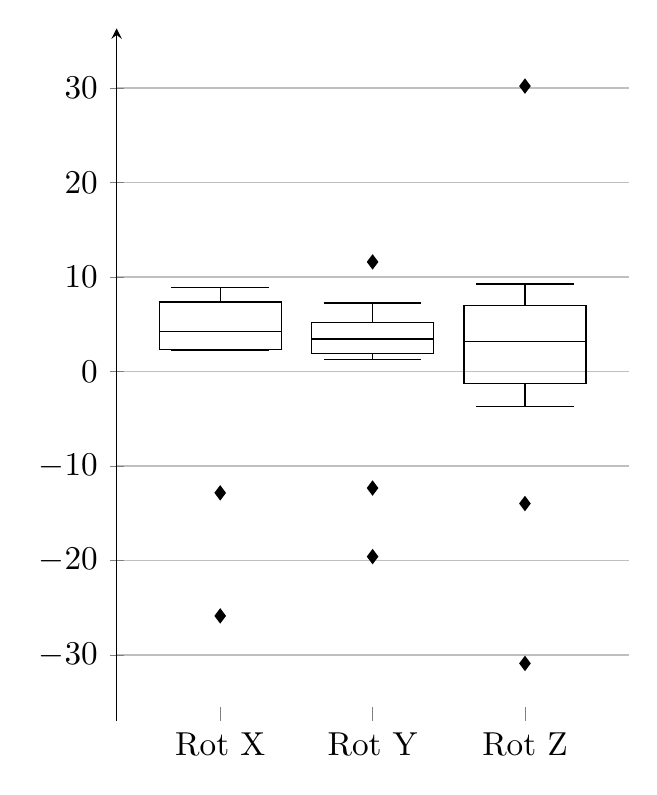
\begin{tikzpicture}[scale=1.2]
\begin{axis}[
boxplot/draw direction=y,
x axis line style={opacity=0},
axis x line*=bottom,
axis y line=left,
enlarge y limits,
ymajorgrids,
y= 0.1cm,
xtick={1,2,3},
xticklabels={Rot X, Rot Y, Rot Z},
]
\addplot+ [
boxplot prepared={
	lower whisker=2.229505,
	lower quartile=2.2854835,
	median= 4.191185,
	upper quartile=7.345289,
	upper whisker=8.907209,
},
] table [row sep=\\,y index=0] {-25.87347\\ -12.85138\\ };
\addplot+ [
boxplot prepared={
	lower whisker=1.262718,
	lower quartile=1.895378,
	median=3.418076,
	upper quartile=5.18264,
	upper whisker=7.253242,
},
] table [row sep=\\,y index=0] {  -19.5975\\ -12.34097\\ 11.59116\\ };
\addplot+ [
boxplot prepared={
	lower whisker=-3.689575,
	lower quartile= -1.261572,
	median=3.170036,
	upper quartile=6.982395,
	upper whisker=9.246979,
},
] table [row sep=\\,y index=0] {-30.89815\\ -13.98067\\ 30.19878\\ };
\end{axis}
\end{tikzpicture} &

%Distanzen zum MittelwertVektor ImageTarget15

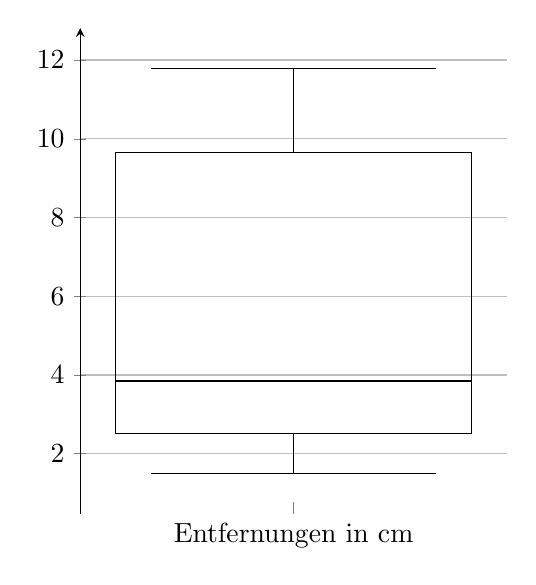
\begin{tikzpicture}
\begin{axis}[
boxplot/draw direction=y,
x axis line style={opacity=0},
axis x line*=bottom,
axis y line=left,
enlarge y limits,
ymajorgrids,
y= 0.5cm,
xtick={1,2,3},
xticklabels={Entfernungen in cm},
]
\addplot+ [
boxplot prepared={
	lower whisker=1.504416,
	lower quartile=2.513568,
	median=3.846865,
	upper quartile=9.6565295,
	upper whisker=11.78049,
},
] coordinates {  };
\end{axis}
\end{tikzpicture} \\

\\
\textbf{ImageTarget16}\\
\\

%Boxplot ImageTarget16
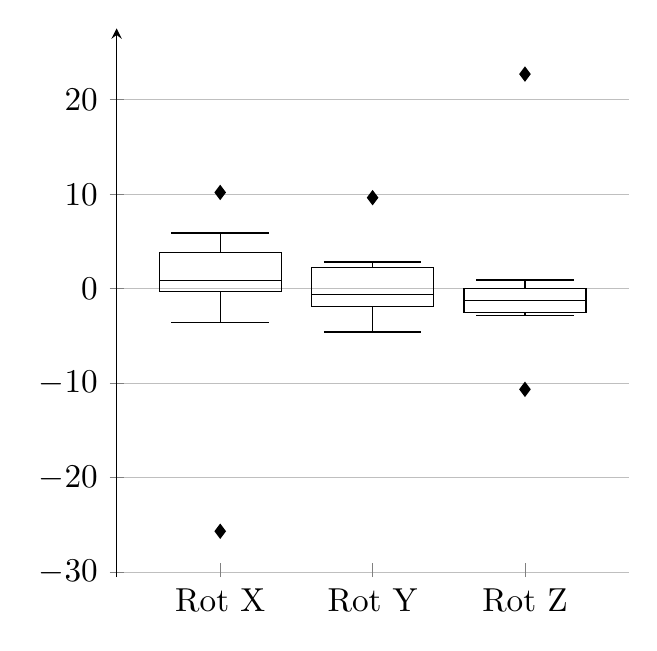
\begin{tikzpicture}[scale=1.2]
\begin{axis}[
boxplot/draw direction=y,
x axis line style={opacity=0},
axis x line*=bottom,
axis y line=left,
enlarge y limits,
ymajorgrids,
y= 0.1cm,
xtick={1,2,3},
xticklabels={Rot X, Rot Y, Rot Z},
]
\addplot+ [
boxplot prepared={
	lower whisker=-3.56192,
	lower quartile=-0.3002014,
	median=0.8713989,
	upper quartile=3.818802,
	upper whisker=5.921753,
},
] table [row sep=\\,y index=0] { -25.65875\\ 10.19672\\ };
\addplot+ [
boxplot prepared={
	lower whisker=-4.566364,
	lower quartile=-1.8923215,
	median=-0.5664179,
	upper quartile=2.2430585,
	upper whisker=2.839506,
},
] table [row sep=\\,y index=0] { 9.645788\\ };
\addplot+ [
boxplot prepared={
	lower whisker=-2.841705,
	lower quartile=-2.491379,
	median=-1.224731,
	upper quartile=0.0268096935,
	upper whisker=0.9228821,
},
] table [row sep=\\,y index=0] {22.72686\\ -10.63632\\ };
\end{axis}
\end{tikzpicture} &

%Distanzen zum MittelwertVektor ImageTarget16
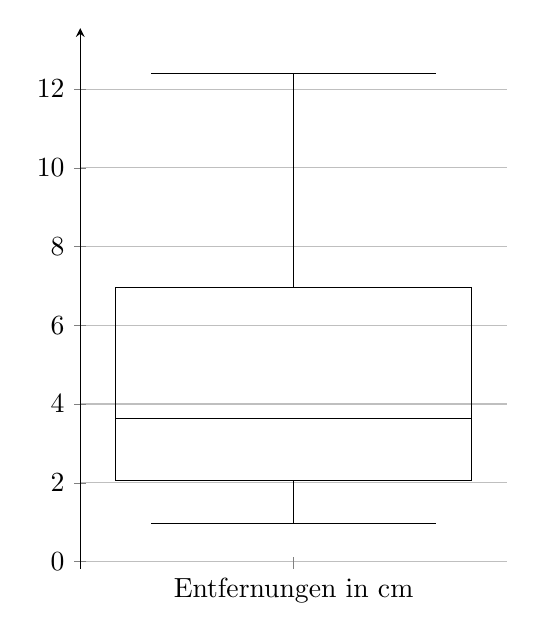
\begin{tikzpicture}
\begin{axis}[
boxplot/draw direction=y,
x axis line style={opacity=0},
axis x line*=bottom,
axis y line=left,
enlarge y limits,
ymajorgrids,
y=0.5cm,
xtick={1,2,3},
xticklabels={Entfernungen in cm},
]
\addplot+ [
boxplot prepared={
	lower whisker=0.009595037*100,
	lower quartile=0.020684825*100,
	median=0.03628322*100,
	upper quartile=0.06965393*100,
	upper whisker=0.1240142*100,
},
] coordinates {  };
\end{axis}
\end{tikzpicture}
\end{tabular}
\caption[Box-Plots pro ImageTarget]{links: Euler-Winkel zwischen den Quaternionen der Nutzerkalibrierungen und des gemittelten Quaternions, rechts: Distanz zwischen den Positionen der Nutzerkalibierungen und der gemittelten Position}
	\label{fig:5.1}
\end{figure}
\end{center} 
\chapter{\iflanguage{english}{Conclusion}{Diskussion}}
\label{cha:conclusion}


What is the outcome of your evaluation?
\begin{itemize}
\item 
\end{itemize}


Did it meet the required goals defined in chapter \ref{cha:introduction}? Why/Why not?


How can future work improve on your work?
\begin{itemize}
\item Bessere Targets
\item Bessere Positionierung
\item Algorithmus, der Erkennt, wenn Target falsch getrackt wird (bspw dadurch, dass der winkel in dem es erkannt wird plötzlich stark anders ist)
\end{itemize}

\cleardoublepage
\listoffigures
\addcontentsline{toc}{chapter}{List of Figures}
%\listofalgorithms
%\addcontentsline{toc}{chapter}{List of Algorithms}
\cleardoublepage

%% --------------------
%% |   Bibliography   |
%% --------------------
\newpage
\addcontentsline{toc}{chapter}{Bibliography}
\bibliography{bibliography}
\bibliographystyle{IEEEtran}

\appendix

\begin{appendices}
\chapter{Evaluation Erklärungstext}
\label{appendix: a}
\setboolean{@twoside}{false}
\includepdf[pages=-, offset=75 -75]{EvaluationExplanation.pdf}
\chapter{Evaluation Fragebogen}
\label{appendix: b}
\setboolean{@twoside}{false}
\includepdf[pages=-, offset=75 -75]{EvaluationFragebogen.pdf}
\chapter{Evaluation Fragebogen Antworten}
\label{appendix: c}
\setboolean{@twoside}{false}
\includepdf[pages=-, offset=75 -75, angle = 90]{FragebogenAntworten.pdf}
\end{appendices}
\end{document}
